\iftoggle{portrait}{
\vfill
  \begin{center}
  \begin{tabular}{cc}
  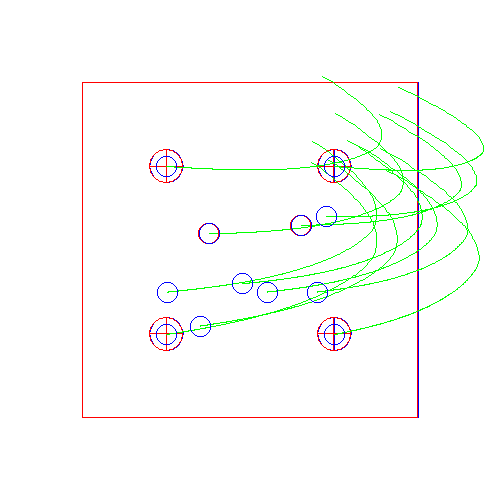
\includegraphics[height=0.1\textheight]{figures/plots/ex5cimage.png}&
  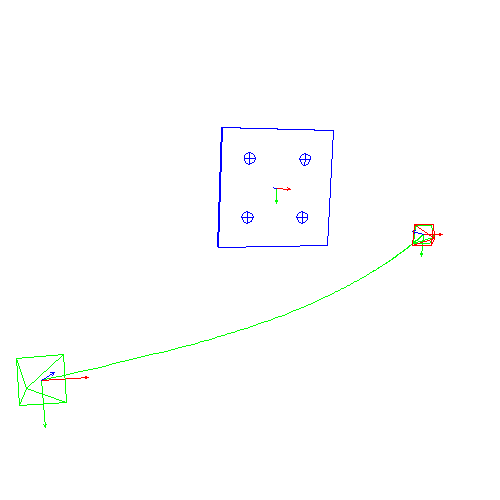
\includegraphics[height=0.1\textheight]{figures/plots/ex5cscene.png}\\
  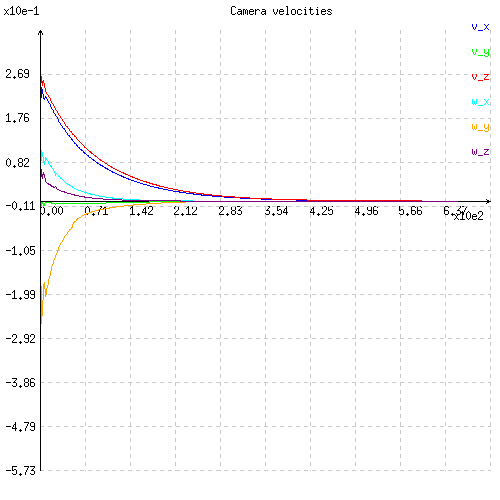
\includegraphics[height=0.1\textheight]{figures/plots/ex5cvelocity.png}&
  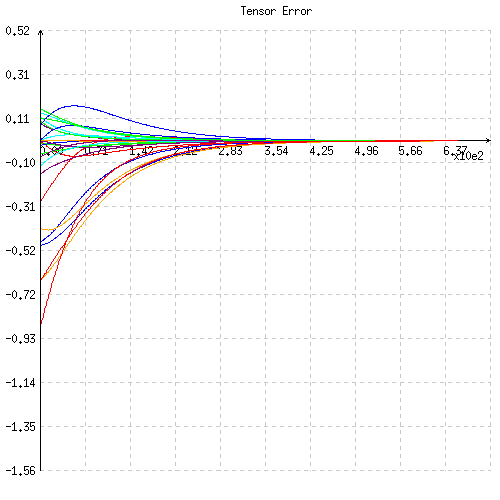
\includegraphics[height=0.1\textheight]{figures/plots/ex5cerror.png}\\
  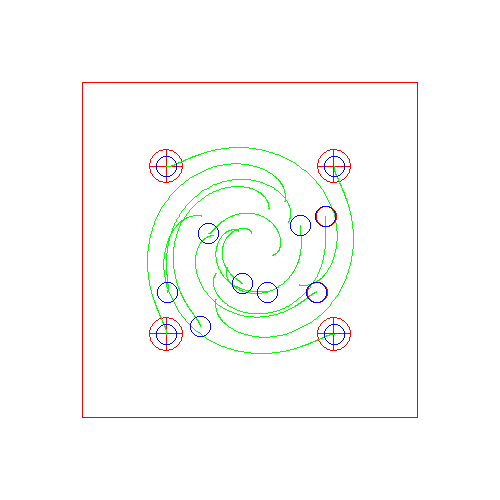
\includegraphics[height=0.1\textheight]{figures/plots/ex4cimage.png}&
  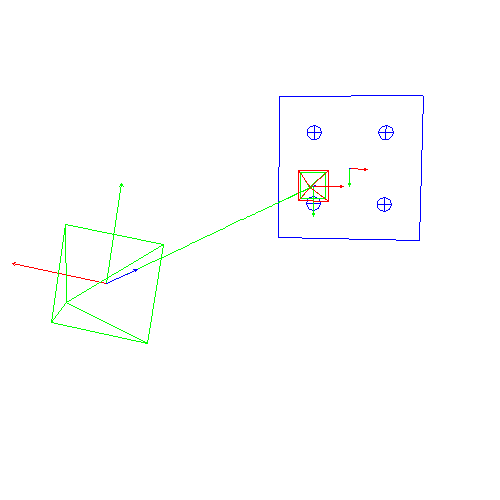
\includegraphics[height=0.1\textheight]{figures/plots/ex4cscene.png}\\
  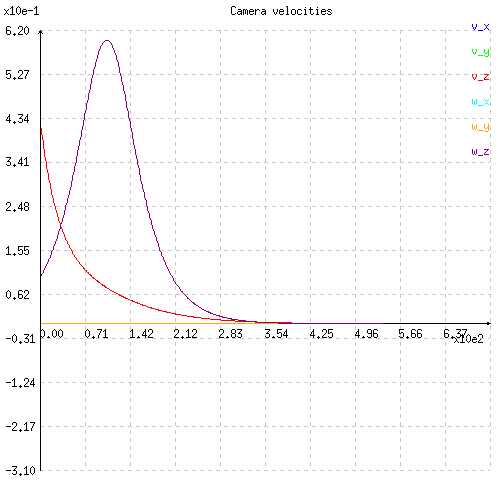
\includegraphics[height=0.1\textheight]{figures/plots/ex4cvelocity.png}&
  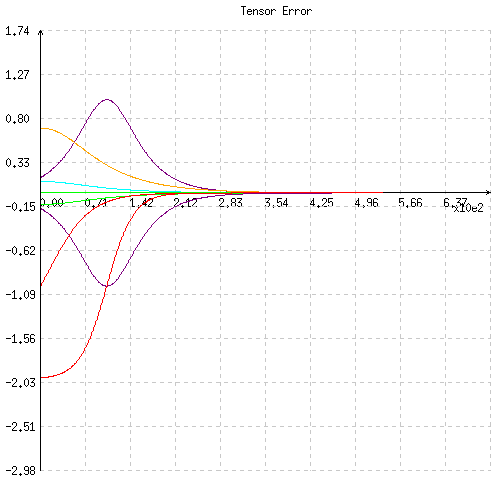
\includegraphics[height=0.1\textheight]{figures/plots/ex4cerror.png}\\
  \end{tabular}
  \end{center}
\vfill
}{
\vfill
\begin{center}
  \begin{tabular}{cc}
  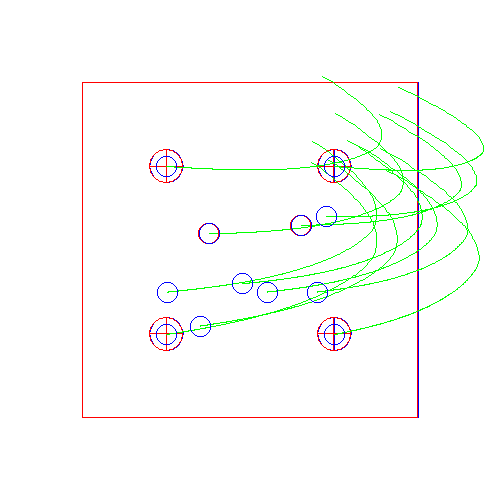
\includegraphics[height=0.15\textheight]{figures/plots/ex5cimage.png}&
  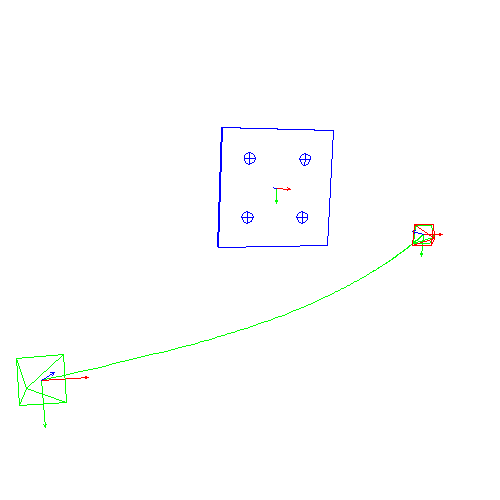
\includegraphics[height=0.15\textheight]{figures/plots/ex5cscene.png}\\
  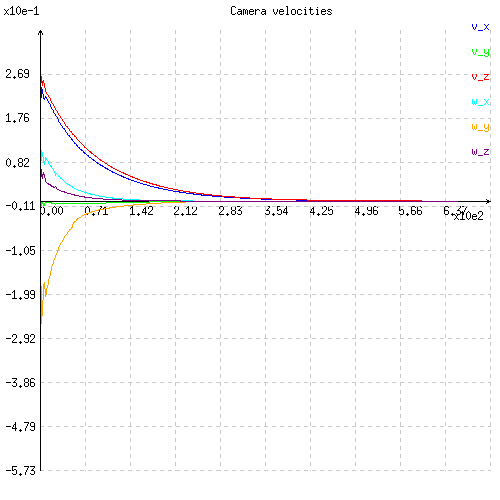
\includegraphics[height=0.15\textheight]{figures/plots/ex5cvelocity.png}&
  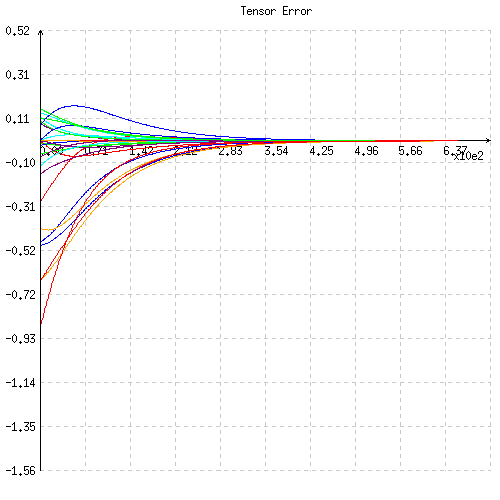
\includegraphics[height=0.15\textheight]{figures/plots/ex5cerror.png}\\
  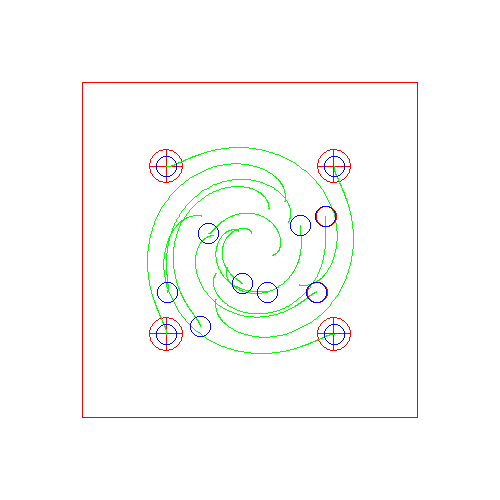
\includegraphics[height=0.15\textheight]{figures/plots/ex4cimage.png}&
  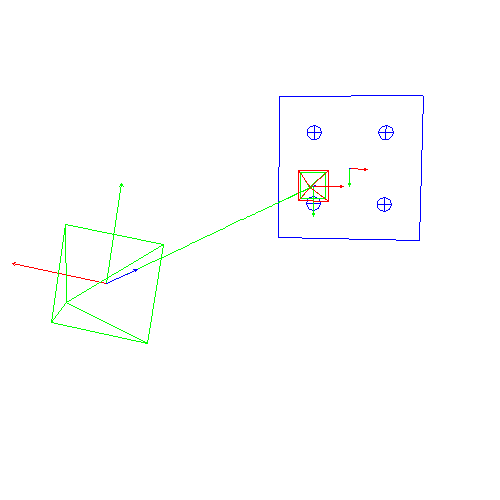
\includegraphics[height=0.15\textheight]{figures/plots/ex4cscene.png}\\
  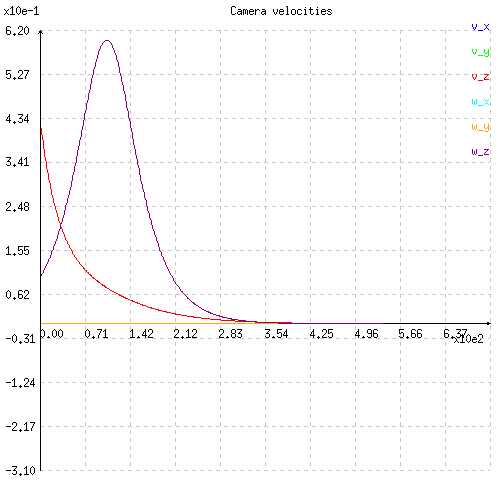
\includegraphics[height=0.15\textheight]{figures/plots/ex4cvelocity.png}&
  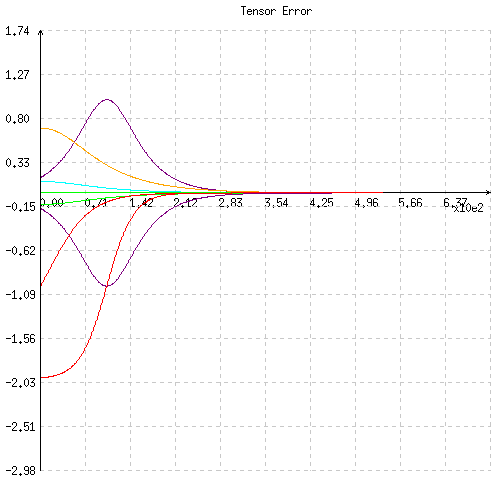
\includegraphics[height=0.15\textheight]{figures/plots/ex4cerror.png}\\
  \end{tabular}
\end{center}
\vfill
}
\begin{enumerate}\compresslist
  \item The approach is working practically with very satisfactory results.
  \item Does not suffer from some of the problems existing in IBVS methods namely the retreat problem.
  \item In the interaction matrix, we have a decoupling between the translational velocities, means smooth camera trajectories for the motion in the 3D space.
\end{enumerate}
However, the \textcolor{lightblue}{initial rotation matrix} is a parameter that needs to be estimated.
